% Chapter 4

\chapter{Architecture}

\label{ch:architecture}

%----------------------------------------------------------------------------------------

\section{Overview}\label{sec:overview}

\tangible{} is implemented as a single Python package, without any external
dependencies.

The architecture of \tangible{} can be categorized into four different parts: The
\hyperref[sec:ast]{abstract syntax tree (AST)}, \hyperref[sec:backends]{code
generation backends}, \hyperref[sec:shapes]{shapes} and
\hyperref[sec:utils]{utils}.

\vspace{7mm}

\begin{figure}[H]
	\centering
	\definecolor{BackendsColor}{RGB}{116,143,204}
\definecolor{AstColor}{RGB}{199,108,107}
\definecolor{ShapesColor}{RGB}{227,225,107}
\definecolor{UtilsColor}{RGB}{118,219,125}

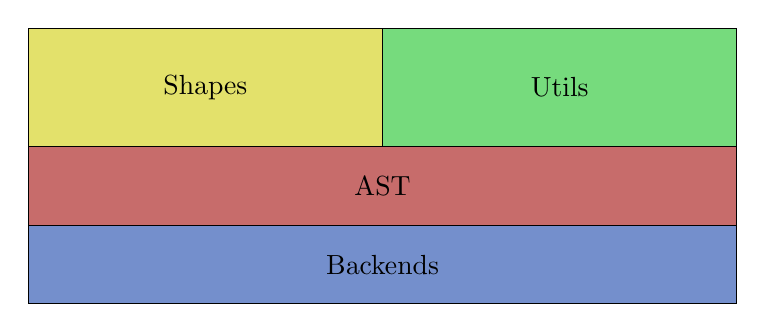
\begin{tikzpicture}
	\filldraw [fill=BackendsColor] (0,0) rectangle node [align=center] {Backends} (9,1) ;
	\filldraw [fill=AstColor] (0,1) rectangle node [align=center] {AST} (9,2);
	\filldraw [fill=ShapesColor] (0,2) rectangle node [align=center] {Shapes} (4.5,3.5);
	\filldraw [fill=UtilsColor] (4.5,2) rectangle node [align=center] {Utils} (9,3.5);
\end{tikzpicture}

	\caption{Architecture Diagram}
	\label{img:architecture}
\end{figure}

%----------------------------------------------------------------------------------------

\section{AST}\label{sec:ast}

The \texttt{ast.py} module provides the objects for the abstract syntax tree
(AST) for \tangible{}. All AST objects extend a single base class called
\texttt{AST}. This base class is responsible for three things:

\begin{itemize}
	\item It provides a single base type to use for type checking, e.g.
		\texttt{isinstance(mysubclass, ast.AST)}.
	\item It overrides the \texttt{\_\_eq\_\_} and \texttt{\_\_ne\_\_} methods in
		a way that all subclasses are compared by value (using
		\texttt{self.\_\_dict\_\_}), and not by identity.
	\item It provides a \texttt{\_\_repr\_\_} implementation that displays both
		the class name as well as the object memory address, which simplifies
		debugging.
\end{itemize}

\noindent The module contains the following classes:

\subsection*{Base Class}
\stepcounter{subsection}\addcontentsline{toc}{subsection}{\thesubsection\hspace*{1.19em}Base Class}

\begin{itemize}
	\item \texttt{AST}: The base shape for all AST elements, as described above.
\end{itemize}

\subsection*{2D Shapes}
\stepcounter{subsection}\addcontentsline{toc}{subsection}{\thesubsection\hspace*{1.19em}2D Shapes}

\begin{itemize}
	\item \texttt{Circle}: A circle shape with a specified radius.
	\item \texttt{CircleSector}: A circle sector shape (pizza slice) with a
		specified radius and angle.
	\item \texttt{Rectangle}: A rectangular shape with a specified width and
		height.
	\item \texttt{Polygon}: A polygon shape made from a list of 2D coordinates.
\end{itemize}

\subsection*{3D Shapes}
\stepcounter{subsection}\addcontentsline{toc}{subsection}{\thesubsection\hspace*{1.19em}3D Shapes}

\begin{itemize}
	\item \texttt{Cube}: A cube with a specified width, height and depth.
	\item \texttt{Sphere}: A sphere with a specified radius.
	\item \texttt{Cylinder}: A cylinder with a height and top/bottom radii.
	\item \texttt{Polyhedron}: An arbitrary 3D shape made from connected triangles
		or quads.
\end{itemize}

\subsection*{Transformations}
\stepcounter{subsection}\addcontentsline{toc}{subsection}{\thesubsection\hspace*{1.19em}Transformations}

\begin{itemize}
	\item \texttt{Translate}: Used to translate an object.
	\item \texttt{Rotate}: Used to rotate an object.
	\item \texttt{Scale}: Used to scale an object.
	\item \texttt{Mirror}: Used to mirror an object.
\end{itemize}

\subsection*{Boolean Operations}
\stepcounter{subsection}\addcontentsline{toc}{subsection}{\thesubsection\hspace*{1.19em}Boolean Operations}

\begin{itemize}
	\item \texttt{Union}: Combine multiple shapes into a single shape.
	\item \texttt{Difference}: A boolean difference of two or more shapes.
	\item \texttt{Intersection}: A boolean intersection of two or more shapes.
\end{itemize}

\subsection*{Extrusions}
\stepcounter{subsection}\addcontentsline{toc}{subsection}{\thesubsection\hspace*{1.19em}Extrusions}

\begin{itemize}
	\item \texttt{LinearExtrusion}: Extrude a 2D object linearly along the z axis.
	\item \texttt{RotateExtrusion}: Extrude a 2D object around the z axis. 
\end{itemize}

%----------------------------------------------------------------------------------------

\section{Backends}\label{sec:backends}

The backends are responsible for code generation. They receive an
\hyperref[sec:ast]{AST} instance, traverse it and emit backend specific code.

At the time of this writing, only one backend has been implemented: The OpenSCAD
backend. But it's be very easy to add additional backends in the future.

\subsection{Creating Custom Backends}

To be valid, a custom backend simply needs to implement the following interface:

\vspace{.5\baselineskip}

\begin{pythoncode}
class CustomBackend(object):
    def __init__(self, ast):
        """Initialize backend using the provided AST."""
    def generate(self):
        """Generate code from AST and return it
        as a unicode string."""
\end{pythoncode}

\noindent The code generated by a backend is returned as a unicode string. It
can then be printed to the terminal or used for further processing.


TODO: cross-reference to implementation details

%----------------------------------------------------------------------------------------

\section{Shapes}\label{sec:shapes}

The \texttt{shapes} package is a key component of \tangible{}. It provides a
hierarchical collection of pre-defined shapes that can be used directly to
generate three dimensional data visualizations.

\begin{figure}[H]
	\centering
	\definecolor{ShapesColor}{RGB}{227,225,107}

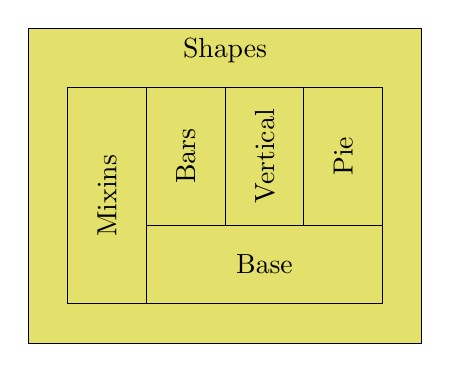
\begin{tikzpicture}

	% Main rectangles

	\filldraw [fill=ShapesColor] (0,0) rectangle (5,4);

	% Inner rectangles

	\draw (1.5,0.5) rectangle node {Base} (4.5,1.5);
	\draw (1.5,1.5) rectangle node [rotate=90] {Bars} (2.5,3.25);
	\draw (2.5,1.5) rectangle node [rotate=90] {Vertical} (3.5,3.25);
	\draw (3.5,1.5) rectangle node [rotate=90] {Pie} (4.5,3.25);
	\draw (0.5,0.5) rectangle node [rotate=90] {Mixins} (1.5,3.25);

	% Labels

	\node [below] at (2.5,4) {Shapes};

\end{tikzpicture}

	\caption{Shapes Architecture}
	\label{img:shapes}
\end{figure}

%----------------------------------------------------------------------------------------

\section{Utils}\label{sec:utils}
